
%(BEGIN_QUESTION)
% Copyright 2011, Tony R. Kuphaldt, released under the Creative Commons Attribution License (v 1.0)
% This means you may do almost anything with this work of mine, so long as you give me proper credit

An instrument technician is asked to physically remove a low oil pressure switch from service in order to perform a routine calibration check on it, while bypassing the automated PLC shutdown system so that the machine will still run while the oil pressure switch is pulled out of service.  The portion of the PLC program handling this automatic shutoff function appears here:

$$\includegraphics[width=15.5cm]{i03580x01.eps}$$

First, identify the ``normal'' status for each of the real-world process switch's electrical contacts (NO or NC), based on the switch descriptions and the PLC program as it is shown:

\begin{itemize}
\item{} Oil pressure switch contacts = {\it NO} or {\it NC}?
\vskip 5pt
\item{} Oil temp switch contacts = {\it NO} or {\it NC}?
\vskip 5pt
\item{} Coolant level switch contacts = {\it NO} or {\it NC}?
\vskip 5pt
\item{} Vibration switch contacts = {\it NO} or {\it NC}?
\end{itemize}

\vskip 10pt

Suppose this technician decides to force the {\tt Shutdown} bit inside the PLC's memory to a low (``0'') state in order to allow the temporary removal of the oil pressure switch.  Recommend a better way this technician could have bypassed the switch's safety function other than forcing the {\tt Shutdown} bit, and also explain why.

\underbar{file i03580}
%(END_QUESTION)





%(BEGIN_ANSWER)

{\it 1 point for each correct NO/NC answer:}

\begin{itemize}
\item{} Oil pressure switch contacts = {\bf NO}
\item{} Oil temp switch contacts = {\bf NC}
\item{} Coolant level switch contacts = {\bf NO}
\item{} Vibration switch contacts = {\bf NO}
\end{itemize}

{\it 3 points for alternative, 3 points for explanation:}

A better way would have been to force the oil pressure switch's input bit to a ``1'' state (or jumper the switch contacts at the most convenient terminal block).  This way, all the other safety switches are still doing their job, able to shut down the machine if something goes wrong.

%(END_ANSWER)





%(BEGIN_NOTES)

{\bf This question is intended for exams only and not worksheets!}.

%(END_NOTES)

